\documentclass[12pt, twoside]{article}
%\documentclass[12pt, twoside]{article}
\usepackage[letterpaper, margin=1in, headsep=0.2in]{geometry}
\setlength{\headheight}{0.6in}
%\usepackage[english]{babel}
\usepackage[utf8]{inputenc}
\usepackage{microtype}
\usepackage{amsmath}
\usepackage{amssymb}
%\usepackage{amsfonts}
\usepackage[nomessages]{fp} %\FPeval{\var-name}{2*sin(pi/6)}
\usepackage{siunitx} %units in math. eg 20\milli\meter
\usepackage{yhmath} % for arcs, overparenth command
\usepackage{tikz} %graphics
\usetikzlibrary{quotes, angles, arrows, arrows.meta}
\usepackage{pgfplots}
\usepgfplotslibrary{fillbetween}
\pgfplotsset{compat=1.16}
\usepackage{graphicx} %consider setting \graphicspath{{images/}}
\usepackage{parskip} %no paragraph indent
\usepackage{enumitem}
\usepackage{multicol}
\usepackage{venndiagram}

\usepackage{fancyhdr}
\pagestyle{fancy}
\fancyhf{}
\renewcommand{\headrulewidth}{0pt} % disable the underline of the header
\raggedbottom
\hfuzz=2mm %suppresses overfull box warnings

\usepackage{hyperref}

\fancyhead[LO]{La Scuola d'Italia / Dr.\ Huson / IB Math 12 (a) \\* 17 November 2026}
\fancyhead[RO]{\fbox{\begin{minipage}{6cm}\footnotesize Nickname:\\[0.5cm]\end{minipage}}}
\fancyfoot[C]{\thepage}

\begin{document}
%======================== Version (a) ========================
\subsubsection*{3.6 Quiz: Periodic Functions}

Problems 1 and 2: \textbf{no calculator}. Problems 3 and 4: a calculator is
allowed. Give answers exactly, or correct to three significant figures.
Diagrams are not to scale.

\begin{enumerate}[itemsep=0.15cm]

%--- Problem 1: Graph of f(x) = 3sin(2x) - 2: max and min, period, a, b, d; dashed graph g = f(x + pi/4): sign of the shift [9 marks] ---
%--- Source: Original (AA SL 2.11, 3.7); no calculator ---
\item[1.] [Maximum mark: 9] \hfill \textbf{No calculator}

The solid curve is the graph of $y = f(x)$, where $f(x) = a\sin(bx) + d$,
for $0 \le x \le \pi$, and $a,\ b > 0$. The dashed curve is the graph of
$y = g(x)$: it is the graph of $f$ translated horizontally by
$\dfrac{\pi}{4}$.

\begin{center}
\begin{tikzpicture}
\begin{axis}[
  axis lines=left,
  xlabel={$x$}, ylabel={$y$},
  xlabel style={at={(axis description cs:1,0)}, anchor=north west},
  ylabel style={at={(axis description cs:0,1)}, anchor=south east, rotate=-90},
  xmin=0, xmax=3.3, ymin=-6, ymax=2.5,
  xtick={0.3927,0.7854,1.1781,1.5708,1.9635,2.3562,2.7489,3.1416},
  xticklabels={$\frac{\pi}{8}$,$\frac{\pi}{4}$,$\frac{3\pi}{8}$,$\frac{\pi}{2}$,
    $\frac{5\pi}{8}$,$\frac{3\pi}{4}$,$\frac{7\pi}{8}$,$\pi$},
  ytick={-6,-5,...,2},
  grid=major, grid style={line width=0.2pt, gray!40},
  tick label style={font=\small},
  width=12.5cm, height=5.6cm, clip=false,
]
  \draw[thin] (axis cs:0,0) -- (axis cs:3.3,0);
  \addplot[very thick, domain=0:3.1416, samples=200] {3*sin(deg(2*x)) - 2};
  \addplot[thick, dashed, domain=0:3.1416, samples=200] {3*cos(deg(2*x)) - 2};
  \addplot[only marks, mark=*, mark size=1.8pt] coordinates {(0.7854,1) (2.3562,-5)};
  \node[anchor=south, fill=white, inner sep=1pt, font=\small] at (axis cs:0.7854,1.3) {$\left(\frac{\pi}{4},\ 1\right)$};
  \node[anchor=north, fill=white, inner sep=1pt, font=\small] at (axis cs:2.3562,-5.25) {$\left(\frac{3\pi}{4},\ -5\right)$};
  \node[anchor=west, font=\small] at (axis cs:3.18,-2) {$y = f(x)$};
  \node[anchor=west, font=\small] at (axis cs:3.18,1) {$y = g(x)$};
\end{axis}
\end{tikzpicture}
\end{center}

\begin{enumerate}[itemsep=0.1cm]
  \item Write down the maximum value and the minimum value of $f$.
  \hfill [2]
  \item Write down the period of $f$. \hfill [1]
  \item Find the value of $a$, of $b$ and of $d$. \hfill [4]
  \item State whether $g(x) = f\!\left(x + \dfrac{\pi}{4}\right)$ or
  $g(x) = f\!\left(x - \dfrac{\pi}{4}\right)$. Give a reason for your
  answer. \hfill [2]
\end{enumerate}

\begin{tikzpicture}
  \draw (-0.6,0) rectangle (14.6,6.6);
  \foreach \y in {1,2,...,6} \draw[dotted] (0,\y)--(14.1,\y);
\end{tikzpicture}

\newpage

%--- Problem 2: Unit circle: 2pi/3 to degrees, exact coordinates of P; 315 deg to radians, exact coordinates of Q; sin(theta) = 2/3 in quadrant II, cos and tan by sin^2 + cos^2 = 1 [10 marks] ---
%--- Source: Original (AA SL 3.4, 3.5, 3.6); no-calculator parallel of 2-6Q version (a) unit-circle problem ---
\item[2.] [Maximum mark: 10] \hfill \textbf{No calculator}

\begin{minipage}[t]{0.5\linewidth}
The diagram shows the unit circle, centre $O$. Angles are measured
anticlockwise from the positive $x$-axis.

Point $P$ is at angle $\dfrac{2\pi}{3}$ and point $Q$ is at angle
$315^\circ$.
\end{minipage}
\hfill
\begin{minipage}[t]{0.46\linewidth}
\vspace{0pt}
\centering
\begin{tikzpicture}[scale=2.0]
  \draw[->] (-1.3,0) -- (1.4,0) node[right] {$x$};
  \draw[->] (0,-1.12) -- (0,1.15) node[right] {$y$};
  \draw[thick] (0,0) circle (1);
  \coordinate (O) at (0,0);
  \coordinate (P) at (120:1);
  \coordinate (Q) at (315:1);
  \draw (O) -- (P);
  \draw (O) -- (Q);
  \fill (P) circle (0.7pt);
  \fill (Q) circle (0.7pt);
  \draw (0.3,0) arc (0:120:0.3);
  \node at (60:0.48) {\footnotesize $\frac{2\pi}{3}$};
  \draw (0.14,0) arc (0:315:0.14);
  \node at (225:0.42) {\footnotesize $315^\circ$};
  \node[above left] at (P) {$P$};
  \node[below right] at (Q) {$Q$};
  \node at (155:0.2) {\footnotesize $O$};
\end{tikzpicture}
\end{minipage}

\begin{enumerate}[itemsep=0.1cm]
  \item Write $\dfrac{2\pi}{3}$ in degrees. \hfill [1]
  \item Write down the exact coordinates of $P$. \hfill [2]
  \item Write $315^\circ$ in radians, as an exact multiple of $\pi$.
  \hfill [1]
  \item Write down the exact coordinates of $Q$. \hfill [2]
\end{enumerate}

The angle $\theta$ satisfies $\sin\theta = \dfrac{2}{3}$ and
$\dfrac{\pi}{2} < \theta < \pi$.

\begin{enumerate}[itemsep=0.1cm]
  \item[(e)] Use the identity $\sin^{2}\theta + \cos^{2}\theta = 1$ to
  find the exact value of $\cos\theta$. \hfill [3]
  \item[(f)] Find the exact value of $\tan\theta$. \hfill [1]
\end{enumerate}

\begin{tikzpicture}
  \draw (-0.6,0) rectangle (14.6,8.7);
  \foreach \y in {1,2,...,8} \draw[dotted] (0,\y)--(14.1,\y);
\end{tikzpicture}

\newpage

%--- Problem 3: Quadrilateral ABCD split by diagonal AC: cosine rule for AC (obtuse angle), sine rule for AD, area of the quadrilateral [9 marks] ---
%--- Source: Original (AA SL 3.2); parallel of 2-6Q version (b) Problem 3 with the sine rule in triangle ACD ---
\item[3.] [Maximum mark: 9] \hfill \textbf{Calculator allowed}

\begin{minipage}[t]{0.55\linewidth}
The diagram shows quadrilateral $ABCD$, with diagonal $[AC]$.

$AB = 7\,\text{cm}$, $BC = 9\,\text{cm}$ and $A\hat{B}C = 110^\circ$.

$A\hat{C}D = 48^\circ$ and $A\hat{D}C = 75^\circ$.
\end{minipage}
\hfill
\begin{minipage}[t]{0.41\linewidth}
\vspace{0pt}
\centering
\begin{tikzpicture}[scale=0.42]
  \coordinate (A) at (0,0);
  \coordinate (B) at (5.362,-4.5);
  \coordinate (C) at (13.157,0);
  \coordinate (D) at (5.513,8.489);
  \draw[thick] (A) -- (B) -- (C) -- (D) -- cycle;
  \draw[dashed] (A) -- (C);
  \draw pic["$110^\circ$", draw, angle radius=0.45cm, angle eccentricity=2.0] {angle = C--B--A};
  \draw pic["$48^\circ$", draw, angle radius=0.7cm, angle eccentricity=1.6] {angle = D--C--A};
  \draw pic["$75^\circ$", draw, angle radius=0.5cm, angle eccentricity=1.8] {angle = A--D--C};
  \node[left] at (A) {$A$};
  \node[below] at (B) {$B$};
  \node[right] at (C) {$C$};
  \node[above] at (D) {$D$};
  \node[below left] at (2.68,-2.25) {$7\,\text{cm}$};
  \node[below right] at (9.26,-2.25) {$9\,\text{cm}$};
\end{tikzpicture}
\end{minipage}

\begin{enumerate}[itemsep=0.1cm]
  \item Find $AC$. \hfill [3]
  \item Find $AD$. \hfill [3]
  \item Find the area of quadrilateral $ABCD$. \hfill [3]
\end{enumerate}

\begin{tikzpicture}
  \draw (-0.6,0) rectangle (14.6,10.9);
  \foreach \y in {1,2,...,10} \draw[dotted] (0,\y)--(14.1,\y);
\end{tikzpicture}

\newpage

%--- Problem 4: Daylight in New York and Palermo, t in days: a, d, b, c of a sine model from the solstices; Palermo p, q; minutes of extra daylight today; days with less than 10 hours in Palermo [12 marks] ---
%--- Source: Original (AA SL 2.11, 3.7); solstice day lengths rounded from the sunrise equation (NYC 40.7 N, Palermo 38.1 N) ---
\item[4.] [Maximum mark: 12] \hfill \textbf{Calculator allowed}

The hours of daylight in New York are modelled by
$N(t) = a\sin\bigl(b(t - c)\bigr) + d$, where $t$ is the number of days
after 31 December ($t = 1$ is 1 January), $a, b, c, d > 0$ and $c < 365$.
The period of the model is $365$ days. The longest day, 21 June
($t = 172$), has $15.1$ hours of daylight; the shortest day, 21 December
($t = 355$), has $9.3$ hours.

\begin{enumerate}[itemsep=0.05cm]
  \item Find the value of $a$ and the value of $d$. \hfill [2]
  \item Find the value of $b$. \hfill [1]
  \item Find the value of $c$. \hfill [2]
\end{enumerate}

The daylight in Palermo, Sicily, can be modelled by
$P(t) = p\sin\bigl(b(t - c)\bigr) + q$, with the same values of $b$ and
$c$. Palermo's longest day has $14.8$ hours of daylight and its shortest
day has $9.5$ hours.

\begin{enumerate}[itemsep=0.05cm]
  \item[(d)] Find the value of $p$ and the value of $q$. \hfill [2]
  \item[(e)] Today is 17 November ($t = 321$). Find how many more minutes
  of daylight Palermo has than New York today. \hfill [2]
  \item[(f)] Find the length of time, in days, during which Palermo has
  fewer than $10$ hours of daylight. \hfill [3]
\end{enumerate}

\begin{tikzpicture}
  \draw (-0.6,0) rectangle (14.6,10.7);
  \foreach \y in {1,2,...,10} \draw[dotted] (0,\y)--(14.1,\y);
\end{tikzpicture}

\end{enumerate}

\newpage

%======================== Version (b) ========================
\fancyhead[LO]{La Scuola d'Italia / Dr.\ Huson / IB Math 12 (b) \\* 17 November 2026}
\subsubsection*{3.6 Quiz: Periodic Functions}

Problems 1 and 2: \textbf{no calculator}. Problems 3 and 4: a calculator is
allowed. Give answers exactly, or correct to three significant figures.
Diagrams are not to scale.

\begin{enumerate}[itemsep=0.15cm]

%--- Problem 1: Unit circle: 4pi/3 to degrees, exact coordinates of P; 135 deg to radians, exact coordinates of Q; sin(theta) = -2/5 in quadrant IV, cos and tan by sin^2 + cos^2 = 1 [10 marks] ---
%--- Source: Original (AA SL 3.4, 3.5, 3.6); parallel of version (a) Problem 2 ---
\item[1.] [Maximum mark: 10] \hfill \textbf{No calculator}

\begin{minipage}[t]{0.5\linewidth}
The diagram shows the unit circle, centre $O$. Angles are measured
anticlockwise from the positive $x$-axis.

Point $P$ is at angle $\dfrac{4\pi}{3}$ and point $Q$ is at angle
$135^\circ$.
\end{minipage}
\hfill
\begin{minipage}[t]{0.46\linewidth}
\vspace{0pt}
\centering
\begin{tikzpicture}[scale=2.0]
  \draw[->] (-1.3,0) -- (1.4,0) node[right] {$x$};
  \draw[->] (0,-1.12) -- (0,1.15) node[right] {$y$};
  \draw[thick] (0,0) circle (1);
  \coordinate (O) at (0,0);
  \coordinate (P) at (240:1);
  \coordinate (Q) at (135:1);
  \draw (O) -- (P);
  \draw (O) -- (Q);
  \fill (P) circle (0.7pt);
  \fill (Q) circle (0.7pt);
  \draw (0.14,0) arc (0:240:0.14);
  \node at (208:0.42) {\footnotesize $\frac{4\pi}{3}$};
  \draw (0.3,0) arc (0:135:0.3);
  \node at (62:0.5) {\footnotesize $135^\circ$};
  \node[below left] at (P) {$P$};
  \node[above left] at (Q) {$Q$};
  \node[below right] at (O) {\footnotesize $O$};
\end{tikzpicture}
\end{minipage}

\begin{enumerate}[itemsep=0.1cm]
  \item Write $\dfrac{4\pi}{3}$ in degrees. \hfill [1]
  \item Write down the exact coordinates of $P$. \hfill [2]
  \item Write $135^\circ$ in radians, as an exact multiple of $\pi$.
  \hfill [1]
  \item Write down the exact coordinates of $Q$. \hfill [2]
\end{enumerate}

The angle $\theta$ satisfies $\sin\theta = -\dfrac{2}{5}$ and
$\dfrac{3\pi}{2} < \theta < 2\pi$.

\begin{enumerate}[itemsep=0.1cm]
  \item[(e)] Use the identity $\sin^{2}\theta + \cos^{2}\theta = 1$ to
  find the exact value of $\cos\theta$. \hfill [3]
  \item[(f)] Find the exact value of $\tan\theta$. \hfill [1]
\end{enumerate}

\begin{tikzpicture}
  \draw (-0.6,0) rectangle (14.6,6.6);
  \foreach \y in {1,2,...,6} \draw[dotted] (0,\y)--(14.1,\y);
\end{tikzpicture}

\newpage

%--- Problem 2: Graph of f(x) = 4sin(2x) + 1: max and min, period, a, b, d; dashed graph g = f(x - pi/4): sign of the shift [9 marks] ---
%--- Source: Original (AA SL 2.11, 3.7); parallel of version (a) Problem 1 (shift to the right here) ---
\item[2.] [Maximum mark: 9] \hfill \textbf{No calculator}

The solid curve is the graph of $y = f(x)$, where $f(x) = a\sin(bx) + d$,
for $0 \le x \le \pi$, and $a,\ b > 0$. The dashed curve is the graph of
$y = g(x)$: it is the graph of $f$ translated horizontally by
$\dfrac{\pi}{4}$.

\begin{center}
\begin{tikzpicture}
\begin{axis}[
  axis lines=left,
  xlabel={$x$}, ylabel={$y$},
  xlabel style={at={(axis description cs:1,0)}, anchor=north west},
  ylabel style={at={(axis description cs:0,1)}, anchor=south east, rotate=-90},
  xmin=0, xmax=3.3, ymin=-4, ymax=6.5,
  xtick={0.3927,0.7854,1.1781,1.5708,1.9635,2.3562,2.7489,3.1416},
  xticklabels={$\frac{\pi}{8}$,$\frac{\pi}{4}$,$\frac{3\pi}{8}$,$\frac{\pi}{2}$,
    $\frac{5\pi}{8}$,$\frac{3\pi}{4}$,$\frac{7\pi}{8}$,$\pi$},
  ytick={-4,-3,...,6},
  grid=major, grid style={line width=0.2pt, gray!40},
  tick label style={font=\small},
  width=12.5cm, height=5.6cm, clip=false,
]
  \draw[thin] (axis cs:0,0) -- (axis cs:3.3,0);
  \addplot[very thick, domain=0:3.1416, samples=200] {4*sin(deg(2*x)) + 1};
  \addplot[thick, dashed, domain=0:3.1416, samples=200] {-4*cos(deg(2*x)) + 1};
  \addplot[only marks, mark=*, mark size=1.8pt] coordinates {(0.7854,5) (2.3562,-3)};
  \node[anchor=south, fill=white, inner sep=1pt, font=\small] at (axis cs:0.7854,5.3) {$\left(\frac{\pi}{4},\ 5\right)$};
  \node[anchor=north, fill=white, inner sep=1pt, font=\small] at (axis cs:2.3562,-3.25) {$\left(\frac{3\pi}{4},\ -3\right)$};
  \node[anchor=west, font=\small] at (axis cs:3.18,1) {$y = f(x)$};
  \node[anchor=west, font=\small] at (axis cs:3.18,-3) {$y = g(x)$};
\end{axis}
\end{tikzpicture}
\end{center}

\begin{enumerate}[itemsep=0.1cm]
  \item Write down the maximum value and the minimum value of $f$.
  \hfill [2]
  \item Write down the period of $f$. \hfill [1]
  \item Find the value of $a$, of $b$ and of $d$. \hfill [4]
  \item State whether $g(x) = f\!\left(x + \dfrac{\pi}{4}\right)$ or
  $g(x) = f\!\left(x - \dfrac{\pi}{4}\right)$. Give a reason for your
  answer. \hfill [2]
\end{enumerate}

\begin{tikzpicture}
  \draw (-0.6,0) rectangle (14.6,8.6);
  \foreach \y in {1,2,...,8} \draw[dotted] (0,\y)--(14.1,\y);
\end{tikzpicture}

\newpage

%--- Problem 3: Quadrilateral ABCD split by diagonal AC: cosine rule for AC (obtuse angle), sine rule for AD, area of the quadrilateral [9 marks] ---
%--- Source: Original (AA SL 3.2); parallel of version (a) Problem 3 ---
\item[3.] [Maximum mark: 9] \hfill \textbf{Calculator allowed}

\begin{minipage}[t]{0.55\linewidth}
The diagram shows quadrilateral $ABCD$, with diagonal $[AC]$.

$AB = 8\,\text{cm}$, $BC = 6\,\text{cm}$ and $A\hat{B}C = 115^\circ$.

$A\hat{C}D = 52^\circ$ and $A\hat{D}C = 70^\circ$.
\end{minipage}
\hfill
\begin{minipage}[t]{0.41\linewidth}
\vspace{0pt}
\centering
\begin{tikzpicture}[scale=0.45]
  \coordinate (A) at (0,0);
  \coordinate (B) at (7.109,-3.669);
  \coordinate (C) at (11.856,0);
  \coordinate (D) at (5.269,8.432);
  \draw[thick] (A) -- (B) -- (C) -- (D) -- cycle;
  \draw[dashed] (A) -- (C);
  \draw pic["$115^\circ$", draw, angle radius=0.45cm, angle eccentricity=2.0] {angle = C--B--A};
  \draw pic["$52^\circ$", draw, angle radius=0.7cm, angle eccentricity=1.6] {angle = D--C--A};
  \draw pic["$70^\circ$", draw, angle radius=0.5cm, angle eccentricity=1.8] {angle = A--D--C};
  \node[left] at (A) {$A$};
  \node[below] at (B) {$B$};
  \node[right] at (C) {$C$};
  \node[above] at (D) {$D$};
  \node[below left] at (3.55,-1.83) {$8\,\text{cm}$};
  \node[below right] at (9.48,-1.83) {$6\,\text{cm}$};
\end{tikzpicture}
\end{minipage}

\begin{enumerate}[itemsep=0.1cm]
  \item Find $AC$. \hfill [3]
  \item Find $AD$. \hfill [3]
  \item Find the area of quadrilateral $ABCD$. \hfill [3]
\end{enumerate}

\begin{tikzpicture}
  \draw (-0.6,0) rectangle (14.6,10.9);
  \foreach \y in {1,2,...,10} \draw[dotted] (0,\y)--(14.1,\y);
\end{tikzpicture}

\newpage

%--- Problem 4: Darkness in New York and Siracusa, t in days: a, d, b, c of a sine model from the solstices; Siracusa p, q; minutes of extra darkness on 1 December; days with more than 13.5 hours of darkness in Siracusa [12 marks] ---
%--- Source: Original (AA SL 2.11, 3.7); parallel of version (a) Problem 4; night lengths = 24 - day lengths from the sunrise equation (NYC 40.7 N, Siracusa 37.1 N) ---
\item[4.] [Maximum mark: 12] \hfill \textbf{Calculator allowed}

The hours of darkness (sunset to sunrise) in New York are modelled by
$D(t) = a\sin\bigl(b(t - c)\bigr) + d$, where $t$ is the number of days
after 31 December ($t = 1$ is 1 January), $a, b, c, d > 0$ and $c < 365$.
The period of the model is $365$ days. The longest night, 21 December
($t = 355$), has $14.7$ hours of darkness; the shortest night, 21 June
($t = 172$), has $8.9$ hours.

\begin{enumerate}[itemsep=0.05cm]
  \item Find the value of $a$ and the value of $d$. \hfill [2]
  \item Find the value of $b$. \hfill [1]
  \item Find the value of $c$. \hfill [2]
\end{enumerate}

The darkness in Siracusa, Sicily, can be modelled by
$S(t) = p\sin\bigl(b(t - c)\bigr) + q$, with the same values of $b$ and
$c$. Siracusa's longest night has $14.4$ hours of darkness and its
shortest night has $9.3$ hours.

\begin{enumerate}[itemsep=0.05cm]
  \item[(d)] Find the value of $p$ and the value of $q$. \hfill [2]
  \item[(e)] Find how many more minutes of darkness New York has than
  Siracusa on 1 December ($t = 335$). \hfill [2]
  \item[(f)] Find the length of time, in days, during which Siracusa has
  more than $13.5$ hours of darkness. \hfill [3]
\end{enumerate}

\begin{tikzpicture}
  \draw (-0.6,0) rectangle (14.6,10.2);
  \foreach \y in {1,2,...,9} \draw[dotted] (0,\y)--(14.1,\y);
\end{tikzpicture}

\end{enumerate}

\newpage

%======================== Version (c) ========================
%--- Scaffolded version (simpler values, hints in every part) ---
\fancyhead[LO]{La Scuola d'Italia / Dr.\ Huson / IB Math 12 (c) \\* 17 November 2026}
\subsubsection*{3.6 Quiz: Periodic Functions}

Problems 1 and 2: \textbf{no calculator}. Problems 3 and 4: a calculator is
allowed. Give answers exactly, or correct to three significant figures.
Diagrams are not to scale.

\begin{enumerate}[itemsep=0.15cm]

%--- Problem 1: Graph of f(x) = 2sin x + 1 with y = sin x dashed: read the y-intercept, max and min points, x-intercepts; d and a from max and min; f(x); describe the stretch and translation [10 marks] ---
%--- Source: Original (AA SL 2.11, 3.7); scaffolded parallel of versions (a) and (b) Problem 1 (vertical stretch and translation only) ---
\item[1.] [Maximum mark: 10] \hfill \textbf{No calculator}

The solid curve is the graph of $y = f(x)$, where $f(x) = a\sin x + d$,
for $0 \le x \le 2\pi$. $A$ is its maximum point and $B$ its minimum point.
The dashed curve is the graph of $y = \sin x$.

\begin{center}
\begin{tikzpicture}
\begin{axis}[
  axis lines=left,
  xlabel={$x$}, ylabel={$y$},
  xlabel style={at={(axis description cs:1,0)}, anchor=north west},
  ylabel style={at={(axis description cs:0,1)}, anchor=south east, rotate=-90},
  xmin=0, xmax=6.6, ymin=-1.5, ymax=3.5,
  xtick={0.5236,1.0472,1.5708,2.0944,2.6180,3.1416,3.6652,4.1888,4.7124,5.2360,5.7596,6.2832},
  xticklabels={$\frac{\pi}{6}$,$\frac{\pi}{3}$,$\frac{\pi}{2}$,$\frac{2\pi}{3}$,$\frac{5\pi}{6}$,$\pi$,
    $\frac{7\pi}{6}$,$\frac{4\pi}{3}$,$\frac{3\pi}{2}$,$\frac{5\pi}{3}$,$\frac{11\pi}{6}$,$2\pi$},
  ytick={-1,0,1,2,3},
  grid=major, grid style={line width=0.2pt, gray!40},
  tick label style={font=\footnotesize},
  width=13cm, height=5.0cm, clip=false,
]
  \draw[thin] (axis cs:0,0) -- (axis cs:6.6,0);
  \addplot[very thick, domain=0:6.2832, samples=200] {2*sin(deg(x)) + 1};
  \addplot[thick, dashed, domain=0:6.2832, samples=200] {sin(deg(x))};
  \addplot[only marks, mark=*, mark size=1.8pt] coordinates {(1.5708,3) (4.7124,-1)};
  \node[anchor=south west, fill=white, inner sep=1pt, font=\small] at (axis cs:1.62,3.0) {$A$};
  \node[anchor=north west, fill=white, inner sep=1pt, font=\small] at (axis cs:4.76,-1.0) {$B$};
  \node[anchor=west, font=\small] at (axis cs:6.33,1.15) {$y = f(x)$};
  \node[anchor=west, font=\small] at (axis cs:6.33,-0.15) {$y = \sin x$};
\end{axis}
\end{tikzpicture}
\end{center}

\begin{enumerate}[itemsep=0.05cm]
  \item Write down the coordinates of the $y$-intercept of $f$. \hfill [1]
  \item Write down the coordinates of $A$ and the coordinates of $B$.
  \hfill [2]
  \item Use the grid to write down the two $x$-intercepts of $f$. \hfill [2]
  \item Find $d = \frac{\text{max} + \text{min}}{2}$ and the amplitude
  $a = \frac{\text{max} - \text{min}}{2}$. \hfill [2]
  \item Write down $f(x)$, using your values of $a$ and $d$. \hfill [1]
  \item Copy and complete: ``The graph of $y = \sin x$ is stretched
  vertically by a scale factor of \underline{\hspace{1cm}}, and then
  translated \underline{\hspace{1cm}} units up, to give $y = f(x)$.''
  \hfill [2]
\end{enumerate}

\begin{tikzpicture}
  \draw (-0.6,0) rectangle (14.6,6.3);
  \foreach \y in {1,2,...,5} \draw[dotted] (0,\y)--(14.1,\y);
\end{tikzpicture}

\newpage

%--- Problem 2: Unit circle (scaffolded): 60 deg to radians; exact cos and sin of pi/3; exact coordinates at pi/4 and at 135 deg by symmetry; sin(theta) = 3/5, theta acute, cos by sin^2 + cos^2 = 1 [9 marks] ---
%--- Source: Original (AA SL 3.4, 3.5, 3.6); scaffolded parallel of versions (a) and (b) unit-circle problem ---
\item[2.] [Maximum mark: 9] \hfill \textbf{No calculator}

\begin{minipage}[t]{0.5\linewidth}
The diagram shows the unit circle, centre $O$. Angles are measured
anticlockwise from the positive $x$-axis.

Point $P$ is at angle $\dfrac{\pi}{4}$ (which is $45^\circ$). Point $Q$ is
at angle $135^\circ$.

A point at angle $\theta$ on the unit circle has coordinates
$(\cos\theta,\ \sin\theta)$.
\end{minipage}
\hfill
\begin{minipage}[t]{0.46\linewidth}
\vspace{0pt}
\centering
\begin{tikzpicture}[scale=2.0]
  \draw[->] (-1.3,0) -- (1.4,0) node[right] {$x$};
  \draw[->] (0,-1.12) -- (0,1.15) node[right] {$y$};
  \draw[thick] (0,0) circle (1);
  \coordinate (O) at (0,0);
  \coordinate (P) at (45:1);
  \coordinate (Q) at (135:1);
  \draw (O) -- (P);
  \draw (O) -- (Q);
  \draw[dotted] (P) -- (0.7071,0);
  \draw[dotted] (Q) -- (-0.7071,0);
  \fill (P) circle (0.7pt);
  \fill (Q) circle (0.7pt);
  \draw (0.3,0) arc (0:45:0.3);
  \node at (22:0.45) {\footnotesize $\frac{\pi}{4}$};
  \draw (0.15,0) arc (0:135:0.15);
  \node at (100:0.32) {\footnotesize $135^\circ$};
  \node[above right] at (P) {$P$};
  \node[above left] at (Q) {$Q$};
  \node[below left] at (O) {\footnotesize $O$};
\end{tikzpicture}
\end{minipage}

\begin{enumerate}[itemsep=0.1cm]
  \item Write $60^\circ$ in radians. Hint: multiply by $\dfrac{\pi}{180}$.
  \hfill [1]
  \item Write down the exact values of $\cos\dfrac{\pi}{3}$ and
  $\sin\dfrac{\pi}{3}$. Hint: use the $30^\circ$--$60^\circ$--$90^\circ$
  triangle. \hfill [2]
  \item Write down the exact coordinates of $P$. \hfill [2]
  \item $Q$ is the reflection of $P$ in the $y$-axis. Write down the exact
  coordinates of $Q$. \hfill [2]
  \item The angle $\theta$ is acute and $\sin\theta = \dfrac{3}{5}$. Use
  $\sin^{2}\theta + \cos^{2}\theta = 1$ to find $\cos\theta$. Hint: start
  with $\left(\dfrac{3}{5}\right)^{2} + \cos^{2}\theta = 1$. \hfill [2]
\end{enumerate}

\begin{tikzpicture}
  \draw (-0.6,0) rectangle (14.6,8.4);
  \foreach \y in {1,2,...,7} \draw[dotted] (0,\y)--(14.1,\y);
\end{tikzpicture}

\newpage

%--- Problem 3: Triangle ABC, SAS with 60 deg (scaffolded): cosine rule for BC = 7, area, sine rule for angle ACB [8 marks] ---
%--- Source: Original (AA SL 3.2); scaffolded parallel of versions (a) and (b) Problem 3 ---
\item[3.] [Maximum mark: 8] \hfill \textbf{Calculator allowed}

\begin{minipage}[t]{0.55\linewidth}
The diagram shows triangle $ABC$, with $AB = 5\,\text{cm}$,
$AC = 8\,\text{cm}$ and $B\hat{A}C = 60^\circ$.

Your calculator must be in \textbf{degree} mode for this problem.
\end{minipage}
\hfill
\begin{minipage}[t]{0.41\linewidth}
\vspace{0pt}
\centering
\begin{tikzpicture}[scale=0.55]
  \coordinate (A) at (0,0);
  \coordinate (B) at (2.5,4.330);
  \coordinate (C) at (8,0);
  \draw[thick] (A) -- (B) -- (C) -- cycle;
  \draw pic["$60^\circ$", draw, angle radius=0.5cm, angle eccentricity=1.7] {angle = C--A--B};
  \node[below left] at (A) {$A$};
  \node[above] at (B) {$B$};
  \node[below right] at (C) {$C$};
  \node[left] at (1.25,2.17) {$5\,\text{cm}$};
  \node[below] at (4,0) {$8\,\text{cm}$};
\end{tikzpicture}
\end{minipage}

\begin{enumerate}[itemsep=0.1cm]
  \item Use the cosine rule, $BC^{2} = AB^{2} + AC^{2} - 2(AB)(AC)\cos A$,
  to find $BC$. \hfill [3]
  \item Use $\text{Area} = \dfrac{1}{2}(AB)(AC)\sin A$ to find the area of
  the triangle. \hfill [2]
  \item Use the sine rule, $\dfrac{\sin C}{AB} = \dfrac{\sin A}{BC}$, to
  find $A\hat{C}B$. \hfill [3]
\end{enumerate}

\begin{tikzpicture}
  \draw (-0.6,0) rectangle (14.6,13.2);
  \foreach \y in {1,2,...,12} \draw[dotted] (0,\y)--(14.1,\y);
\end{tikzpicture}

\newpage

%--- Problem 4: Daylight models for New York and Palermo, t in months (scaffolded): max and min from a and d; period; N(10.5) in radian mode; Palermo max and min; minutes of extra daylight on the shortest day [10 marks] ---
%--- Source: Original (AA SL 2.11, 3.7); scaffolded parallel of version (a) Problem 4 ---
\item[4.] [Maximum mark: 10] \hfill \textbf{Calculator allowed}

The number of hours of daylight in New York can be modelled by
\[
  N(t) = 2.9\sin\left(\frac{\pi}{6}(t - 2.7)\right) + 12.2,
\]
where $t$ is the time in months after 1 January.

Your calculator must be in \textbf{radian} mode for this problem.

\begin{enumerate}[itemsep=0.1cm]
  \item The largest value of $\sin$ is $1$ and the smallest is $-1$. Write
  down the maximum and the minimum number of hours of daylight in New York.
  \hfill [2]
  \item The period of $y = a\sin\bigl(b(t - c)\bigr) + d$ is
  $\dfrac{2\pi}{b}$. Find the period of $N$, in months. \hfill [2]
  \item Today is 17 November ($t = 10.5$). Find $N(10.5)$, the number of
  hours of daylight in New York today. \hfill [2]
\end{enumerate}

The number of hours of daylight in Palermo, Sicily, can be modelled by
\[
  P(t) = 2.65\sin\left(\frac{\pi}{6}(t - 2.7)\right) + 12.15.
\]

\begin{enumerate}[itemsep=0.1cm]
  \item[(d)] Write down the maximum and the minimum number of hours of
  daylight in Palermo. \hfill [2]
  \item[(e)] On the shortest day of the year, how many more minutes of
  daylight does Palermo have than New York? \hfill [2]
\end{enumerate}

\begin{tikzpicture}
  \draw (-0.6,0) rectangle (14.6,8.4);
  \foreach \y in {1,2,...,7} \draw[dotted] (0,\y)--(14.1,\y);
\end{tikzpicture}

\end{enumerate}
\end{document}
